%*
%* Seven Kingdoms: Ancient Adversaries
%*
%* Copyright 1997,1998 Enlight Software Ltd.
%* Copyright 2018 Timothy Rink
%*
%* This program is free software: you can redistribute it and/or modify
%* it under the terms of the GNU General Public License as published by
%* the Free Software Foundation, either version 2 of the License, or
%* (at your option) any later version.
%*
%* This program is distributed in the hope that it will be useful,
%* but WITHOUT ANY WARRANTY; without even the implied warranty of
%* MERCHANTABILITY or FITNESS FOR A PARTICULAR PURPOSE.  See the
%* GNU General Public License for more details.
%*
%* You should have received a copy of the GNU General Public License
%* along with this program.  If not, see <http://www.gnu.org/licenses/>.
%*
%*

\chapter{The Information Interface}

\index{game!interface}
\index{interface of game}

\textgoth{\Huge{O}}n the top of your screen, you will see all of the information necessary to keep your budding Empire under your firm grip.

\begin{center}
	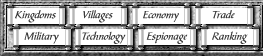
\includegraphics[width=0.7\linewidth]{Iscrolls}
\end{center}

Beginning on the Left, you will see the Scrolls. \textbf{Click} on a Scroll to see the detailed information inside each. You may also access these Scrolls by pressing the \textbf{F1} through \textbf{F8} keys on your keyboard.

Once you have opened one of these Scrolls, it can be closed by \textbf{Clicking} it again or by pressing the \textbf{Esc} key on your keyboard.

\section{Kingdoms}

\index{kingdoms scroll}

\textgoth{\Huge{O}}pen this Scroll if you want to see information on all of the world’s Kingdoms that you have discovered so far in your explorations of the world.

\begin{center}
	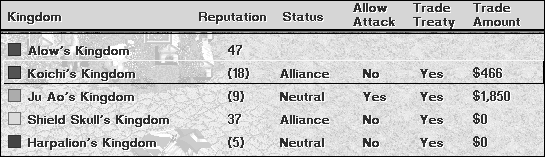
\includegraphics[width=0.9\linewidth]{Ikingdoms}
\end{center}

Below this area, you will see three buttons that will take you into three different areas. These are \textbf{Information}, \textbf{Diplomacy}, and the \textbf{Diplomatic Log}.

\subsection{Information}

\index{information on the relationship with other kingdom}

\textgoth{\Huge{U}}nder the \textbf{Information Button}, you will see more detailed information on your relationship with the selected Kingdom.

\begin{center}
	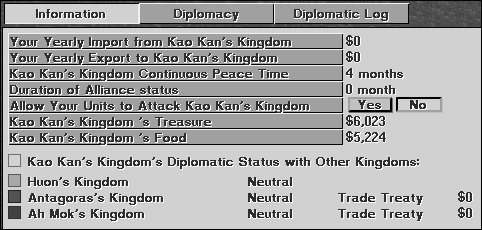
\includegraphics[width=0.9\linewidth]{Ikingdoms_information}
\end{center}

You will also be able to see the diplomatic relationships that the other Kingdoms have with each other.

For Kingdoms that are your allies, you will be able to see their cash and food reserves as well.

The Yearly Imports and Exports are figured for the preceding 365 days.

\subsubsection{Allow Attack}

\index{allowing attack}

\textgoth{\Huge{B}}y \textbf{Clicking} the \textbf{Yes} or \textbf{No Buttons} in this section, you will be able to manually select whether or not your troops will be allowed to attack units or structures of the selected Kingdom. The game will begin with the default setting of Yes.

The Yes or No option will be set automatically in the following situations:

\begin{changemargin}{.1cm}{0cm} % Larger indent here.

\index{attacking!Allow Attack option}
	
When you form a Friendly or Alliance Treaty with another Kingdom, your Allow Attack option will be automatically set to No. You will be unable to attack any units or structures unless you manually change the setting.

When you enter into a War with a Kingdom, your Allow Attack option will be automatically set to Yes.

If you accept a Cease Fire in a war, the Allow Attack option with the other signatory will be changed to No.
\end{changemargin}

It would be very wise of you to set the Allow Attack option to No for every Kingdom that you are not planning to attack. This will prevent the sometimes unavoidable incidents of friendly-fire casualties from blowing up into full-scale war. If Allow Attack is set to No, the other Kingdom will understand that any such incident was just a mistake.

\subsection{Diplomacy and Diplomatic Log}

\textgoth{\Huge{F}}or these two buttons, see the detailed descriptions in \textbf{Chapter 13}.

\section{Villages}

\index{villages scroll}

\textgoth{\Huge{O}}pening this Scroll will give you detailed information on all of your Villages. This includes Village Population, the number of Peasants, Village Loyalty, and a list of the various Nationalities living in the Village.

\textbf{Double-Clicking} on the name of a Village will center it on your screen.

In the bottom chart, you will see a detailed list of your Buildings, including their Building Cost, Number, Yearly Upkeep Cost, and Yearly Income (if any) from that Building. The “Yearly” figures are based on the past 365 days.

\section{Economy}

\index{economy scroll}

\textgoth{\Huge{O}}pen this Scroll to see all the information you could wish for on your economy. It will detail all of your income and expenses and the Profit or Loss that you are running at the present time. This includes:

\subsection{Income}

\index{income}

\subsubsection{Sale of Goods}

The amount of sales of Finished Goods to Villagers.

\subsubsection{Exports}

The amount of exports of Raw Materials or Finished Goods to other Kingdoms.

\subsubsection{Taxes}

The amount of Taxes collected from Villagers.

\subsubsection{Recovered Treasure}

The amount of Treasure recovered from the slaying of Frhytans.

\subsubsection{Worker Income}

The income received by your subjects who are working in the firms of other Kingdoms.

\subsubsection{Sale of Buildings}

Your income from the sale of your Factories, Mines, Towers of Science, etc.

\subsubsection{Tribute from other Kingdoms}

Money that you have either forced other Kingdoms to pay you or that they have given in hope of obtaining your good will.

\subsection{Expenses}

\index{expenses}

\subsubsection{General Costs}

The Maintenance costs for all of your Generals.

\subsubsection{Spy Costs}

The Maintenance costs for all of your Spies.

\subsubsection{Other Mobile Human Unit Costs}

The Maintenance costs for all human units except Generals and Spies.

\subsubsection{Caravan Costs}

The Maintenance costs for all of your Caravans.

\subsubsection{Weapons Costs}

The Maintenance costs for all of your Weapons.

\subsubsection{Ships Costs}

The Maintenance costs for all of your Ships.

\subsubsection{Buildings Costs}

The Construction and Maintenance costs for all of your Buildings.

\subsubsection{Training Units}

The Cost of Training all of your units.

\subsubsection{Hiring Units}

The Cost of Hiring units from Inns.

\subsubsection{Honoring Units}

The Cost of Honors given to your units.

\subsubsection{Foreign Worker Salaries}

The money paid to foreigners working in your Buildings.

\subsubsection{Grants to your Villages}

The Cost of your Grants to your Villages.

\subsubsection{Grants to other Villages}

The Cost of your Grants to other Villages.

\subsubsection{Imports}

The Costs of all of your Imports.

\subsubsection{Aid/Tribute to other Kingdoms}

The Money that you have paid in Tribute or given in Aid to other Kingdoms.

\section{Trade}

\index{trade!scroll}

\textgoth{\Huge{I}}nside this Scroll you will see detailed the routing and loads of all of your Caravans and all of your Ships that are being used in Trade. \textbf{Double-Clicking} on a Caravan or a Trader in this menu will center your screen over it.

\section{Military}

\index{military scroll}

\textgoth{\Huge{I}}n this Scroll, you will see your military disposition. It will list your King and all of your Generals and the number of troops that they command. \textbf{Double-Clicking} on the King or a General will center your screen over his location.

\section{Technology}

\index{technology scroll}

\textgoth{\Huge{T}}his Scroll reports on the progress of all of your research projects in all of your Towers of Science.

It also shows the Scrolls of Power that you have acquired and your Greater Beings that are currently active.

\section{Espionage}

\index{espionage scroll}

\textgoth{\Huge{T}}his top-secret Scroll details the activities of all of your spies all over the world. \textbf{Double-Clicking} on a spy’s listing will center the screen over his location.

\section{Ranking}

\index{ranking scroll}

\textgoth{\Huge{T}}his Scroll will show you the rank of your Kingdom against all of the other Kingdoms in a number of categories, such as Population, Military Strength, Economic Strength, Reputation and Fryhtan Battling.

It will also give you a total score by adding up these different categories, show all set Goals and display the total playing time.

\section{State of the Kingdom}

\index{kingdom!state of}
\index{state of kingdom}

\begin{center}
	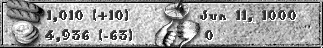
\includegraphics[width=0.7\linewidth]{Ifoodgoldetc}
\end{center}

\textgoth{\Huge{T}}o the right of the Function Scrolls, you will see four icons. These are, on the left: Food and Treasure, and on the right: Date and Reputation.

\subsection{Food}

\index{food}

\textgoth{\Huge{T}}he number in the upper left indicates how much Food is stored in your empire. The number in the parentheses to the right shows how much of a food surplus or deficit you have produced in the past year.

Each person in your kingdom, whether a Peasant, Worker or Mobile Unit, consumes 10 units of food each year. Remember that food is produced by your Peasants. If you do not keep enough Peasants you will run out of food. To maintain a constant food supply, you will need one Peasant toiling in the field for every three subjects of your kingdom.

If your Kingdom runs out of food, prepare for the worst. The Loyalty Levels of all of your units will decrease by one point every five days.

You may request to purchase food from other Kingdoms under the \textbf{Kingdoms Scroll/Diplomacy Button menu}.

\subsection{Treasure}

\index{treasure}

\textgoth{\Huge{T}}he number in the lower left indicates the amount of gold in your treasury. The number in the parenthesis to the right shows how much of a cash surplus or deficit you have incurred in the past year.

It is very important to keep your eyes on your Treasury and your Food supply.

Without money to pay the salaries of your Generals or Mobile units you will see a decrease in their Loyalty.

If you don’t have enough to pay your Spies in foreign Kingdoms, their Loyalty will also decrease. If they are acting as Counterspies in your own Kingdom you will also need to feed them. If you cannot their Loyalty will decrease.

If you can no longer pay foreign workers, they will resign.

If you no longer have enough money to maintain your Weapons or Ships, they will begin losing Hit-Points. If the situation continues, they will completely break down.

If you run out of funds, you will no longer be able to maintain your buildings. They will fall into disrepair and eventually collapse.

\subsection{Calendar}

\index{calendar}

\textgoth{\Huge{I}}t is here that you see the day and year. In a multiplayer game, this may become very important when you and your Allies are synchronizing an attack on another Kingdom.

\subsection{Reputation}

\index{reputation}

\textgoth{\Huge{T}}his number represents the esteem in which your Kingdom is held by the people of the world. A high Reputation level can have many and varied benefits during the long struggle for world domination.

Your Reputation may suffer if you persist in actions that other Kingdoms find to be downright antisocial or if you fail to adequately protect your subjects. The following are the various penalties you will pay for your behavior:

\begin{changemargin}{.5cm}{0cm}
If you attack a Kingdom without first declaring war:

Your Reputation will decrease by 40\% of your target’s Reputation, but only if the target has a positive Reputation.

\textbf{If you declare war on another Kingdom:}

Your Reputation will decrease by 20\% of your target’s Reputation, but only if the target has a positive Reputation.

\textbf{If you terminate an alliance treaty:}

Your Reputation will decrease by 20\% of the target’s Reputation, but only if their Reputation is positive. Note that if you declare war on an ally, your Reputation will decrease twice: once for declaring war and once for terminating an alliance.

\textbf{If you terminate a friendly treaty: }

Your Reputation will decrease by 10\% of the target’s Reputation, but only if the target has a positive Reputation. Note that if you declare war on a Kingdom with which you have a friendly treaty your Reputation will decrease twice; once for declaring war and once for terminating a friendly treaty.

\textbf{If you terminate a trade treaty:}

Your Reputation will decrease by 5\% of the target’s Reputation, but
only if the target has a positive Reputation.

\textbf{Additional Penalties}

\textbf{-10} points for destroying an enemy Caravan.

\textbf{-10} points for Sinking a Trader.
\end{changemargin}

\begin{changemargin}{1cm}{0cm}
Although Caravels and Galleons may be used for trade, they are armed and may, therefore, be sunk without penalty.
\end{changemargin}

\begin{changemargin}{.5cm}{0cm}
\textbf{-3} points if one of your Caravans is destroyed by an enemy.

\textbf{-3} points if one of your Traders is sunk by an enemy.

\textbf{-3} points if one of your Spies is caught Spying.

\textbf{-1} points for each enemy Civilian collaterally damaged in the defense of their town.

\textbf{-0.3} points for each enemy Civilian collaterally damaged in battle.

\textbf{-0.3} points if one of your Civilians is cruelly murdered by an enemy.

Your Reputation will automatically increase by \textbf{+0.5} points per month, and by even more if you are engaged in battling Fryhtans.
\end{changemargin}

Because of the penalties for killing Civilians, you should be very clear on just who is a civilian and who isn’t. If you hold your cursor over an enemy unit, and no small icon pops up, you will know that he is a civilian.

\begin{wrapfigure}{r}{0.5\textwidth}
\vspace{-20pt}
	\begin{center}
		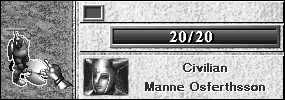
\includegraphics[width=0.4\textwidth]{Ipeasant2}
\end{center}
\vspace{-20pt}
\end{wrapfigure}

If you \textbf{Click} on any unit, you will be shown, as you can see on the right, more details on the unit. \\

\clearpage

\section{Map Modes}

\index{map modes}

\begin{center}
	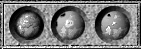
\includegraphics[width=0.4\linewidth]{Imapmode}
\end{center}

\textgoth{\Huge{O}}n the top left of your screen, you will see the three \textbf{World Map Mode Buttons}. These are, left to right: \textbf{Terrain View Button}, \textbf{Borders View Button}, and \textbf{Village View Button}.

\subsection{Terrain View Button}

\index{World Map modes!terrain view}

\textgoth{\Huge{T}}his is the default mode. When \textbf{Clicked}, it will show the World Map in relief and in its natural colors. You will also be able to see Villages, Troop, and Ship movements in the color of their respective Kingdoms.

\subsection{Borders View Button}

\index{World Map modes!border view}

\textgoth{\Huge{T}}he center button has two modes in itself. \textbf{Clicking} on it the first time will show the political borders of each kingdom on the World Map. You may also view all Troop and Ship movements. \textbf{Clicking} on this button a second time will project those political borders onto the main screen area.

Units of other Kingdoms will try to walk around your borders in their travels. This, of course, does not include Caravans or Soldiers who are coming to attack you.

\subsection{Village View Button}

\index{World Map modes!village view}

\textbf{\textgoth{\Huge{C}}licking} on this button will show you a simplified World Map with all Villages and all buildings clearly displayed. You may also view all Troop and Ship movements. Forested areas will not be shown on this map.

\clearpage

\section{Unit Information}

\begin{wrapfigure}{r}{0.5\textwidth}
	\vspace{-20pt}
	\begin{center}
		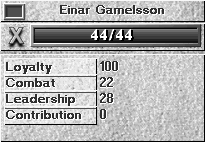
\includegraphics[width=0.4\textwidth]{Iunitinfo}
	\end{center}
	\vspace{-20pt}
\end{wrapfigure}

\textgoth{\Huge{W}}henever you \textbf{Click} on one of your units, you will be presented with information showing that unit’s Color, Name, Hit-Points, Loyalty Level, Combat Skill Level, Leadership Level, and Contribution Total.

Every person in the world of \textit{Seven Kingdoms: Ancient Adversaries} bears a unique name.

To center a selected Person, Weapon, Ship, Caravan, or Building on the main screen, \textbf{Click} on its name.

\section{News}

\index{news}

\textgoth{\Huge{O}}n the bottom of your main screen, you will receive news of happenings from around the world. From the in-game Options menu, you may decide if you want to receive all of the news or just the major happenings.

On the bottom right of your main screen, you will be able to see two small icons.

If you want to clear all of the news from the screen, \textbf{Click} on the 
\includegraphics[width=0.02\linewidth]{Bx} Icon or press the X key on your keyboard.

If you want to view the complete News Log, showing all of the previous news reports, \textbf{Click} on the 
\includegraphics[width=0.02\linewidth]{Bnews} Icon.

Some of the news reports will have a “Go To” Icon in front of them. If you wish to go to the location of the news story, \textbf{Click} on the 
\includegraphics[width=0.02\linewidth]{Bgoto} Icon.